\chapter{Instalacion y Configuracion}

Este Capítulo pretende ser una guía para realizar una exitosa implementación del servidor de producción \footnote{Diferenciamos servidor de producción porque durante el desarrollo las aplicaciones en Django se prueban en un servidor virtual que crea Django para que se pueda correr la aplicación fácilmente, pero esto no es suficiente a la hora de utilizar la aplicación con usuarios finales principalmente por que el servidor de desarrollo no es lo suficientemente potente además de ser lento y consumir demasiados recursos, esta más que nada pensado para que el desarrollador pruebe la aplicación sobre él para así luego pasar a una versión de producción. } la principal consideración es que la implementación será sobre el sistema operativo Windows 7, en caso de querer instalar el sistema en otro sistema operativo, existen algunas diferencias. \\[0.5cm]

\section{Requerimientos}

\subsection{Requerimientos de Hardware}

Cualquier equipo que cumpla con las características para correr Windows 7 es suficiente en términos de requerimientos mínimos de Hardware siempre y cuando el número de usuarios esperados no sea alto, después el resto dependerá de sus necesidades. \\[0.5cm]

\begin{itemize}
    \item Procesador x86, x64 de 1.6 Ghz o superior.
    \item Memoria RAM 1 GB o Superior 
\end{itemize}


\subsection{Requerimientos de Software}


\begin{itemize}
    \item Apache 2.2
    \item PosgreSQL 9.2
    \item Python 2.7.x o Python 2.6.x
    \item Django 1.3.x o Superior
    \item PGAdmin
    \item psycopg2
    \item mod\_wsgi
    \item ReportLab
    \item easy\_thumbnails
    \item django\_extensions
    \item django\_cron
\end{itemize}


\section{Apache}

Existen 2 caminos para instalar Apache, la primera Hacer una instalación limpia de apache, la 2da es cuando no se quiere trastear con tanta configuración por lo que opta por infraestructuras tipo WAMP, LAMP, WAPP, etc. 

\subsection{Instalación en Limpio}

Solo recomiendo este tipo de instalación desde 0 para quienes ya poseen un conocimiento avanzado en cuanto al manejo de servidores. \\[0.5cm]

Descargamos de \url{Apache.org} la última versión disponible, se puede utilizar el siguiente vinculo: \url{http://www.apachehaus.com/cgi-bin/download.plx}.\\[0.5cm]

Crea dos carpetas en la unidad C, la primera de nombre {\bfseries Apache} y la segunda {\bfseries servidor}. Descomprime el archivo descargado y ejecútalo, sigue los pasos de la instalación y de los datos que te piden solo escoge el destino de la instalación, que será la carpeta que creaste en {\bfseries C:\textbackslash Apache}, los otros datos déjalos de la forma predeterminada para configurarlos más tarde. \\[0.5cm]

El programa al instalarse crea un icono en el área de notificación que te permitirá: iniciar, detener y reiniciar Apache; tienes que tener en cuenta que cualquier cambio que hagas en el archivo de configuración no tendrá efecto hasta que reinicies el servidor. \\[0.5cm]

\subsection{Instalación mediante WAMP, LAMP, MAMP, WAPP}

Existen una infinidad de Paquetes precompilados y configurados, con Apache, PHP, PosgreSQL o MySQL y más. \\[0.5cm]
Dichas infraestructuras suelen nombrarse como el acronomico de las herramientas que agrupan por ejemplo:\\[0.5cm]

\begin{itemize}
    \item {\large WAMP {\bfseries W}indows {\bfseries A}pache {\bfseries M}ySQL {\bfseries P}HP}
    \item {\large WAPP  {\bfseries W}indows {\bfseries A}pache {\bfseries P}osgreSQL {\bfseries P}HP}  
    \item {\large LAMP {\bfseries L}inux {\bfseries A}pache {\bfseries M}ySQL {\bfseries P}HP} 
    \item {\large MAMP {\bfseries M}ac OS {\bfseries A}pache {\bfseries M}ySQL {\bfseries P}HP}  
\end{itemize}


Algunas de las distribuciones más usadas disponibles Para Windows son :\\[0.5cm]
\begin{itemize}
    \item WAMP Server \url{http://www.wampserver.com/} (WAMP),
    \item XAMPP \url{http://sourceforge.net/projects/xampp/} 
    \item (WAMP + Perl), Bitnami \url{http://bitnami.com/stack/wapp} (WAPP)
\end{itemize}

Solo nos resta elegir cualquiera de ellas e instalarlas, aparte de la ruta de instalación nos pedirán el usuario y
contraseña para acceder al motor de Base de Datos.

\subsection{Configuración}

Toda la configuración para el funcionamiento de Apache se guarda en un archivo de texto nombrado: {\bfseries httpd.conf} que se encuentra en la ruta {\bfseries C:\textbackslash Apache \textbackslash conf } si realizamos una instalación en limpio o {\bfseries C:\textbackslash WAMP \textbackslash bin \textbackslash  Apache \textbackslash conf } si instalamos el paquete múltiple preconfigurado no es necesario realizar este paso por lo que lo podremos saltar. \\[0.5cm]


Al archivo {\bfseries httpd.conf} lo podemos editar en cualquier editor de texto como Notepad o algo más avanzado como Notepad++, Geany, etc. \\[0.5cm]

Buscamos la línea que dice

\begin{lstlisting}[style=consola, numbers=none]
    Listem LocalHost:80
\end{lstlisting}

Y la Cambiamos por:

\begin{lstlisting}[style=consola, numbers=none]
    Listem 80
\end{lstlisting}

Ahora buscamos la instrucción:

\begin{lstlisting}[style=consola, numbers=none]
    DocumentRoot "C:\xxxxxxxx"
\end{lstlisting}

La Cambiamos por:

\begin{lstlisting}[style=consola, numbers=none]
    DocumentRoot "C:\Servidor"
\end{lstlisting}

Recordar que al inicio de la instalación creamos una carpeta llamada Servidor en la unidad C. Por último solo nos queda reiniciar el servidor Apache e introducir la siguiente dirección \url{http://127.0.0.1} si nos aparece una página {\bfseries It's Work!} felicidades Apache está Funcionando. El problema más común por lo que aveses apache no inicia se debe a que el puerto puede estar siendo utilizado por otra aplicación como Skype, para ello asegúrese antes de que el puerto 80 este libre o utilice otro puerto como el 8080.


\subsection{Instalación de PosgreSQL}

La versión de PostgreSQL que he utilizado durante el desarrollo del sistema es la 9.2.x, quizás cuando leas esto ya halla salido una nueva versión la cual no debería generar inconvenientes además de que es posible que el proceso de instalación pueda variar.\\[0.2cm]
 
El primer paso es descargar el instalador de PostgreSQL para Windows, el cual puedes descargar desde el enlace siguiente \url{http://www.postgresql.org/download/windows}, nos bajara un instalador similar
a {\bfseries postgresql-9.2.3-rc1-windows.exe} lo ejecutamos como administrador.\\[0.2cm]

Si tenemos activado el control de cuentas de usuario nos mostrara una advertencia con el texto "¿Desea permitir que este programa realice cambios en el equipo?", pulsaremos "Sí" para continuar con la instalación de PostgreSQL.\\[0.2cm]

Indicaremos la carpeta de instalacion de PostgreSQL, donde se guardarán los ejecutables, librerías y ficheros de configuración de PostgreSQL en mi caso el directorio es {\bfseries C: \textbackslash PostgreSQL \textbackslash 9.2 }, Indicaremos también la carpeta donde se guardarán los datos por defecto de PostgreSQL {\bfseries C: \textbackslash psql-data }.\\[0.2cm]

Solo nos queda introducir la contraseña para el súper usuario "postgres" \footnote{Puedes cambiar la contraseña y crear un nuevo usuario para aumentar la seguridad del sistema solo recuerda que deberás cambiar la configuración de Django para que este pueda conectarse a la base de datos con un usuario diferente.} que será con el que iniciemos sesión para administrar la base de datos, después podremos crear otros usuarios si es necesario. Además introduciremos el puerto de escucha para la conexión con el servidor PostgreSQL, por defecto el 5432.\\[0.2cm]

Seleccionaremos la configuración regional y comenzara la instalación, con esto PostgreSQL quedara instalado. Si tenemos algún cortafuego (firewall) deberemos abrir el puerto 5432.

\subsection{Creación de la Base de Datos}

Junto con la Instalación de PosgreSQL se instala el PGAdmin III que es una herramienta GUI\footnote{GUI (del inglés \textit{graphical user interface}) es un programa informático que actúa de interfaz de usuario, utilizando un conjunto de imágenes y objetos gráficos para representar la información y acciones disponibles en la interfaz} para administrar el motor de base de Datos. Iniciamos el Programa, desplegaremos "Server Groups", dentro desplegaremos "Servidores" y dentro de éste pulsaremos con el botón derecho del ratón sobre "PostgreSQL 9.0 (localhost:5432), en el menú emergente seleccionaremos "Conectar".

Introduciremos la contraseña para el súper usuario postgres (la contraseña introducida en la instalación).

Pulsaremos con el botón derecho del ratón sobre "Bases de datos", seleccionaremos "Nueva Base de Datos", en la pestaña "Propiedades" introduciremos los siguientes datos:

\begin{itemize}
    \item Nombre: nombre de la base de datos, en nuestro caso "BDSem".
    \item Propietario: seleccionaremos el usuario creado anteriormente "posgres".
    \item Codificado: seleccionaremos UTF8.
    \item Tablespace: seleccionaremos el tablespace creado anteriormente "pg\_default".
    \item Colación: seleccionaremos "Spanish, Argentina".
    \item Tipo carácter: seleccionaremos "Spanish, Argentina".
\end{itemize}

Pulsaremos OK para crear la base de datos, con esto ya tendremos nuestra base de datos aunque vacía, el resto como creación de las Tablas correspondientes necesarias para el proyecto lo haremos más adelante mediante Django.



\section{Instalación de Python}

Para este proyecto se utilizo CPython pero no la versión Oficial url{http://www.python.org} sino la que distribuye Active State \url{http://www.activestate.com} llamada {\bfseries Active Python} la cual provee características adicionales a versión oficial, podremos descargar la ultima versión desde  \url{http://www.activestate.com/activepython/downloads} aunque se recomienda instalar la version 2.7.x para evitar cualquier posible problema ya que es incompatible con las versión 3.x de Python.

\subsection{Probando Python}
Para probar que la instalación haya sido correcta abriremos la Terminal "cmd.exe" y escribiremos:

\begin{lstlisting}[style=consola, numbers=none]
    python
\end{lstlisting} 

Si todo va bien nos deberá aparecer algo similar a:

\begin{figure}[h]
    \centering
    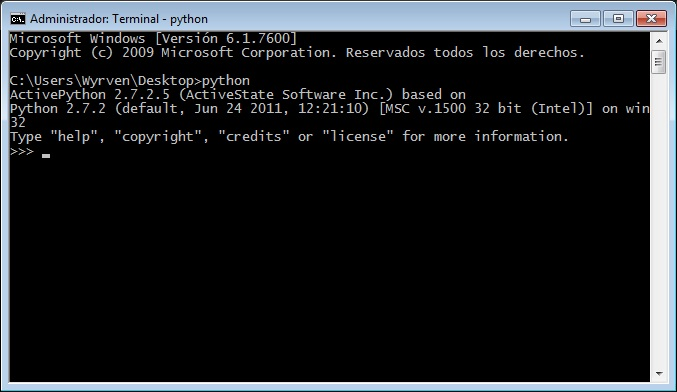
\includegraphics[scale=0.7]{resourse/consola-python.jpg}
    \caption{Ejecutando Python en la Terminal}
    \label{fig:01}
\end{figure}    

En caso contrario deberías revisar que la ruta de Python este dentro de la variable  PATH del sistema.




